\section{Experimentación}

Nuestro equipo de pruebas fue una notebook Lenovo Y40 con procesador Intel\textregistered Core\texttrademark i7-4510U CPU con 2 núcleos físicos y 4 lógicos, corriendo a 2.0 GHz y 16 GB de memoria RAM. Todas las mediciones de tiempo de ejecución fueron tomadas utilizando el TSC (\emph{timestamp counter}), un registro interno del procesador que lleva la cuenta de cuantos ciclos del procesador han pasado desde su último reset. Compilamos la versión en C con el compilador C de GNU Compiler Collection utilizando la opción de optimización \texttt{-O3}. Para cada caso de prueba, corrimos los algoritmos 25 veces y promediamos los tiempos de ejecución, para tener una mejor estimación. En este experimento, compararemos las dos implementaciones del algoritmo. Para esto, utilizamos un conjunto de datos de entrada que consiste en una esfera y una luz que dejamos fijo. Entonces, vamos variando el tamaño de la imagen deseada tomando $i_w \times i_h \in [100000 \dots 2000000]$, para ver si existe la mejora que esperamos con la implementación. En la figura 2 se ven los resultados.\\

\begin{figure}[H]
	\begin{center}
		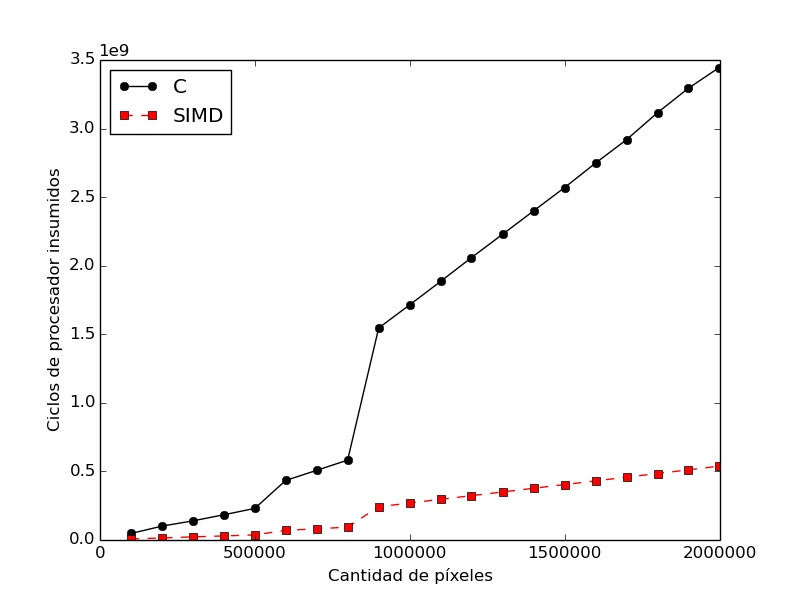
\includegraphics[scale=0.5]{graph1.jpg}
	\end{center}		
	\caption{Tiempo de ejecución del algoritmo de trazado de rayos}
	\label{fig2}
\end{figure}

Ahora vemos los resultados exactos, para poder calcular exactamente la mejora de performance:\\

\begin{center}
\begin{tabular}[H]{|c|c|c|c|}\hline
$i_w \times i_h$ & \textbf{C} & \textbf{SIMD} & \textbf{C/SIMD} \\\hline
99645 & 47412965.4 & 7458009.6 & 6.35\\
199692 & 101101387.08 & 14760852.94 & 6.84\\
299568 & 139660581.06 & 22901589.62 & 6.09\\
399310 & 183821009.3 & 29576126.24 & 6.21\\
499392 & 230551223.58 & 37123983.44 & 6.21\\
598980 & 434228563.54 & 70736674.38 & 6.13\\
699384 & 508383989.28 & 81353151.38 & 6.24\\
798768 & 582486590.68 & 94119090.62 & 6.18\\
898995 & 1545718116.28 & 242396510.46 & 6.37\\
999364 & 1715182797.38 & 269795128.46 & 6.35\\
1099588 & 1887044517.02 & 296972078.78 & 6.35\\
1198272 & 2059100630.34 & 323324739.4 & 6.36\\
1298892 & 2229584118.58 & 350339094.04 & 6.36\\
1398784 & 2399859498.14 & 377197091.18 & 6.36\\	
1498840 & 2569943753.52 & 404182225.46 & 6.35\\
1598700 & 2748590124.28 & 430763849.88 & 6.38\\
1699145 & 2919986197.18 & 458490048.64 & 6.36\\
1798389 & 3115715808.92 & 484714280.96 & 6.42\\
1898063 & 3294098954.12 & 511512759.16 & 6.43\\
1997568 & 3445162034.08 & 538688063.42 & 6.39\\\hline

\end{tabular}
\end{center}
\clearpage
Como vemos en la figura 2, la implementación SIMD es más de 6 veces más rápida que la implementación C. También vemos que la diferencia de performance se mantiene constante cambiando la resolución. Esperabamos que el aumento de performance fuera de $3x$ aproximadamente, ya que en la mayoría de las operaciones, se manejan tres variables al mismo tiempo en vez de una. Entonces, consideramos que esa mejora de la performance mayor se debe al cambio de las funciones a macros y a que, programando a bajo nivel, se puede programar más eficientemente que en C al poner todas las variables en registros y eliminando las que no se necesitan.
También, notamos dos saltos en tiempo de ejecución considerables, a partir de $5 \times 10^6$ píxeles y a partir de $9 \times 10^6$. Consideramos que esto es porque a partir de esos números los datos dejan de caber en la memoria caché del procesador, entonces el programa tarda más tiempo en recuperar los datos de memoria.